\section{Simplifying NTK into atomic units: Roles of gates, weights, width and depth}\label{sec:fc}
In this section, we simply the NTK into atomic units (\Cref{th:main}): we first simplify the \emph{neural path kernel} (NPK) associated with the neural path features into a product of base kernels in \Cref{lm:productkernel} (new result in this paper) and invoke {Theorem $5.1$}, \cite{npk}. 
\subsection{Neural Path Kernel: Composition of Base Kernels}
We will now discuss the properties of \emph{neural path kernel} (NPK) associated with the NPFs defined in \Cref{sec:dual}.  
\begin{definition}
Let $H_{\Theta}(x,x')\eqdef\langle\phi_{x,\Theta},\phi_{x',\Theta} \rangle$ be the NPK.
\end{definition}
\begin{comment}
As a result, it turns out that, depending on the network architecture, the NPK has interesting structure/form. In FC-DNN, the NPK involves product of base kernels (\Cref{def:layerkernel},\Cref{lm:productkernel}) corresponding to the binary gating features of the various layers. In ResNet with $b$ skip connections there are $2^b$ sub-FC-DNNs and the NPK is a sum of the NPKs of these sub-FC-DNNs (\Cref{lm:sumofproduct}). Further, in CNNs due to weight sharing, the NPK has a rotationally invariant form (\Cref{lm:cnnnpk}). In what follows, we define the NPK matrix to be  $H_{\Theta}\eqdef\Phi^\top_{\Theta}\Phi_{\Theta}$, where $\Phi_{\Theta}=(\phi_{x_1,\Theta},\ldots,\phi_{x_n,\Theta})\in\R^{P\times n}$ is the NPF matrix.
\end{comment}
Recall from \Cref{def:nps} that a co-ordinate of NPF can be non-zero only if the corresponding path is active. Consequently, the NPK for a pair of input examples is a similarity measure that depends on the number of paths that are active for both examples. Such common active paths are captured in a quantity denoted by $\Lambda$ defined below.
\begin{definition}\label{def:cnnlambda}
The total number of `active' paths for both $x$ and $x'$ that pass through input node $i$ is defined to be:
{$\Lambda_{\Theta}(i,x,x') \eqdef \left|\{p\in[P]\colon  \Ifeat_0(p)=i, A_{\Theta}(x,p)= A_{\Theta}(x',p)=1\}\right|$}
\end{definition}
%\subsection{NPK of FC-DNN: Product Kernel }
%\input{cnpkexample}
%\subsection{Neural Path Kernel : Similarity based on active sub-networks}
\begin{definition}[Layer-wise Kernel]\label{def:layerkernel} Let $G_{x,\Theta}(\cdot,l)\in\R^w$ be $w$-dimensional feature of the gating values in layer $l$ for input $x\in\R^{\din}$.  Define layer-wise kernels:
\begin{align*}
H^{\text{lyr}}_{l,\Theta}(x,x')\eqdef\ip{G_{x,\Theta}(\cdot,l)G_{x',\Theta}(\cdot,l)}
\end{align*}
\end{definition}
The number of active paths are in turn dependent on the number of active gates in each layer, a fact that endows the NPK with a hierarchical/composite structure. Gates are the basic building blocks, and the gates in a layer form a $w$-dimensional binary feature whose kernels are the base kernels. When the layers are laid out depth-wise, we obtain a product of the base kernels. 
\begin{lemma}[Product Kernel]\label{lm:productkernel}
 Let $H^{\text{fc}}$ denote the NPK of a FC-DNN. Let $D\in\R^{\din\times\din}$ be a diagonal matrix with strictly positive entries, and for $u,u'\in\R^{\din}$ , let $\ip{u,u'}_{D}=\sum_{i=1}^{\din}D(i)u(i)u'(i)$. Then:

$
H^{\text{fc}}_{\Theta}(x,x')= \ip{x,x'}_{\Lambda(\cdot,x,x')}=\ip{x,x'}\cdot\Pi_{l=1}^{d-1}H^{\text{lyr}}_{l,\Theta}(x,x')
$

\end{lemma}
\subsection{Main Theorem: $\text{NTK}^{\text{fixed-gate}}\propto\text{NPK}$}
\begin{assumption}\label{assmp:main}
(i) $\Tv_0$ is statistically independent of $\Tf_0$ (ii) $\Tv_0$ are i.i.d symmetric Bernoulli over $\{-{\sigma},+{\sigma}\}$. 
\end{assumption}

\begin{theorem}\label{th:main} Let $\sigma=\frac{\cscale}{\sqrt{w}}$. Under \Cref{assmp:main}, a $w\ra\infty$, for FC-DGN we have: 
\begin{align*}
\kv_{\Tdgn_0}(x,x')&\stackrel{(a)}\ra d \sigma^{2(d-1)} H^{\text{fc}}_{\Tf_0}(x,x')\\ 
%&\stackrel{(a)}{=} d \sigfc^{2(d-1)}\langle x,x'\rangle\cdot \Pi_{l=1}^{d-1} \left(\frac{\langle G_{x,\Tf_0}(l), G_{x',\Tf_0}(l) \rangle}{w}   \right)\\
%&\stackrel{(a)}\propto \langle x,x'\rangle\cdot \Pi_{l=1}^{d-1} \left(\frac{\langle G_{x,\Tf_0}(l), G_{x',\Tf_0}(l) \rangle}{w}   \right)\\
&\stackrel{(b)}\propto \langle x,x'\rangle\cdot \Pi_{l=1}^{d-1} \frac{H^{\text{lyr}}_{l,\Tf_0}(x,x')}{w}
\end{align*}
\end{theorem}
In \Cref{th:main}, $(a)$ was already shown in {Theorem $5.1$}, \cite{npk}, and $(b)$ follows from \Cref{lm:productkernel}. Also, it is known from prior results \cite{arora2019exact,cao2019generalization} that training and generalisation is characterised by the NTK, and \Cref{th:main} (as well as {Theorem $5.1$}, \cite{npk}) shows that learning with fixed gates is characterised by the NPK. The implications of \Cref{th:main} are listed below.

$\bullet$ \textbf{Role of Weights:}  The weights of the feature network that dictate the NPFs (and hence the NPK) are more critical than the NPV (as long as the NPV is chosen as per \Cref{assmp:main}). Thus, the primary role of the weights is to generate the gates, i.e., the NPFs/NPK. In particular, copying the weights of a pre-trained DNN onto the feature network and training the NPV from scratch recovers the test accuracy of original pre-trained DNN within $1\%$ (see \Cref{sec:exp}). 

$\bullet$ \textbf{Role of Activations:} The ReLU is a special activation, that is, it acts as a gate and the gates themselves are learnt. In particular, learnt gates achieve better test accuracy than random gate (see \Cref{sec:exp}). Also note that, \Cref{th:main} applies to any arbitrary gating, i.e., the $w\ra\infty$ is only binding on the value network, in the case of feature network with finite width, the gates can be \emph{repeated} infinite times to meet the $w\ra\infty$ condition. 

$\bullet$ \textbf{Width} is responsible for averaging (division by $w$) of the base kernels.

$\bullet$ \textbf{Depth} gives rise to a product of base kernels. 

$\bullet$ \textbf{Permutation Invariance:} The NPK is invariant if the layers (as masks) are permuted. This is because the $\Pi_{l=1}^{d-1} \frac{H^{\text{lyr}}_{l,\Tf_0}(x,x')}{w}$ is permutation invariant. We verify this experimentally (see \Cref{sec:exp}).

$\bullet$ \textbf{Constant Inputs:} Even if the input to the value network is set of a constant, i.e., even if $\langle x,x'\rangle$ is made constant, the gates still hold information in the from of $\Pi_{l=1}^{d-1} \frac{H^{\text{lyr}}_{l,\Tf_0}(x,x')}{w}$. We verify this experimentally (see \Cref{sec:exp}).

The points that the gates (i.e., NPFs) are important and that the gates (i.e., NPFs) are learnt were made in prior work \cite{npk}. In this paper, we strengthen these with further experiments (see \Cref{sec:exp}).

\begin{comment}
\subsection{Pictorial Illustration}
\FloatBarrier
\begin{figure}[h]
\centering
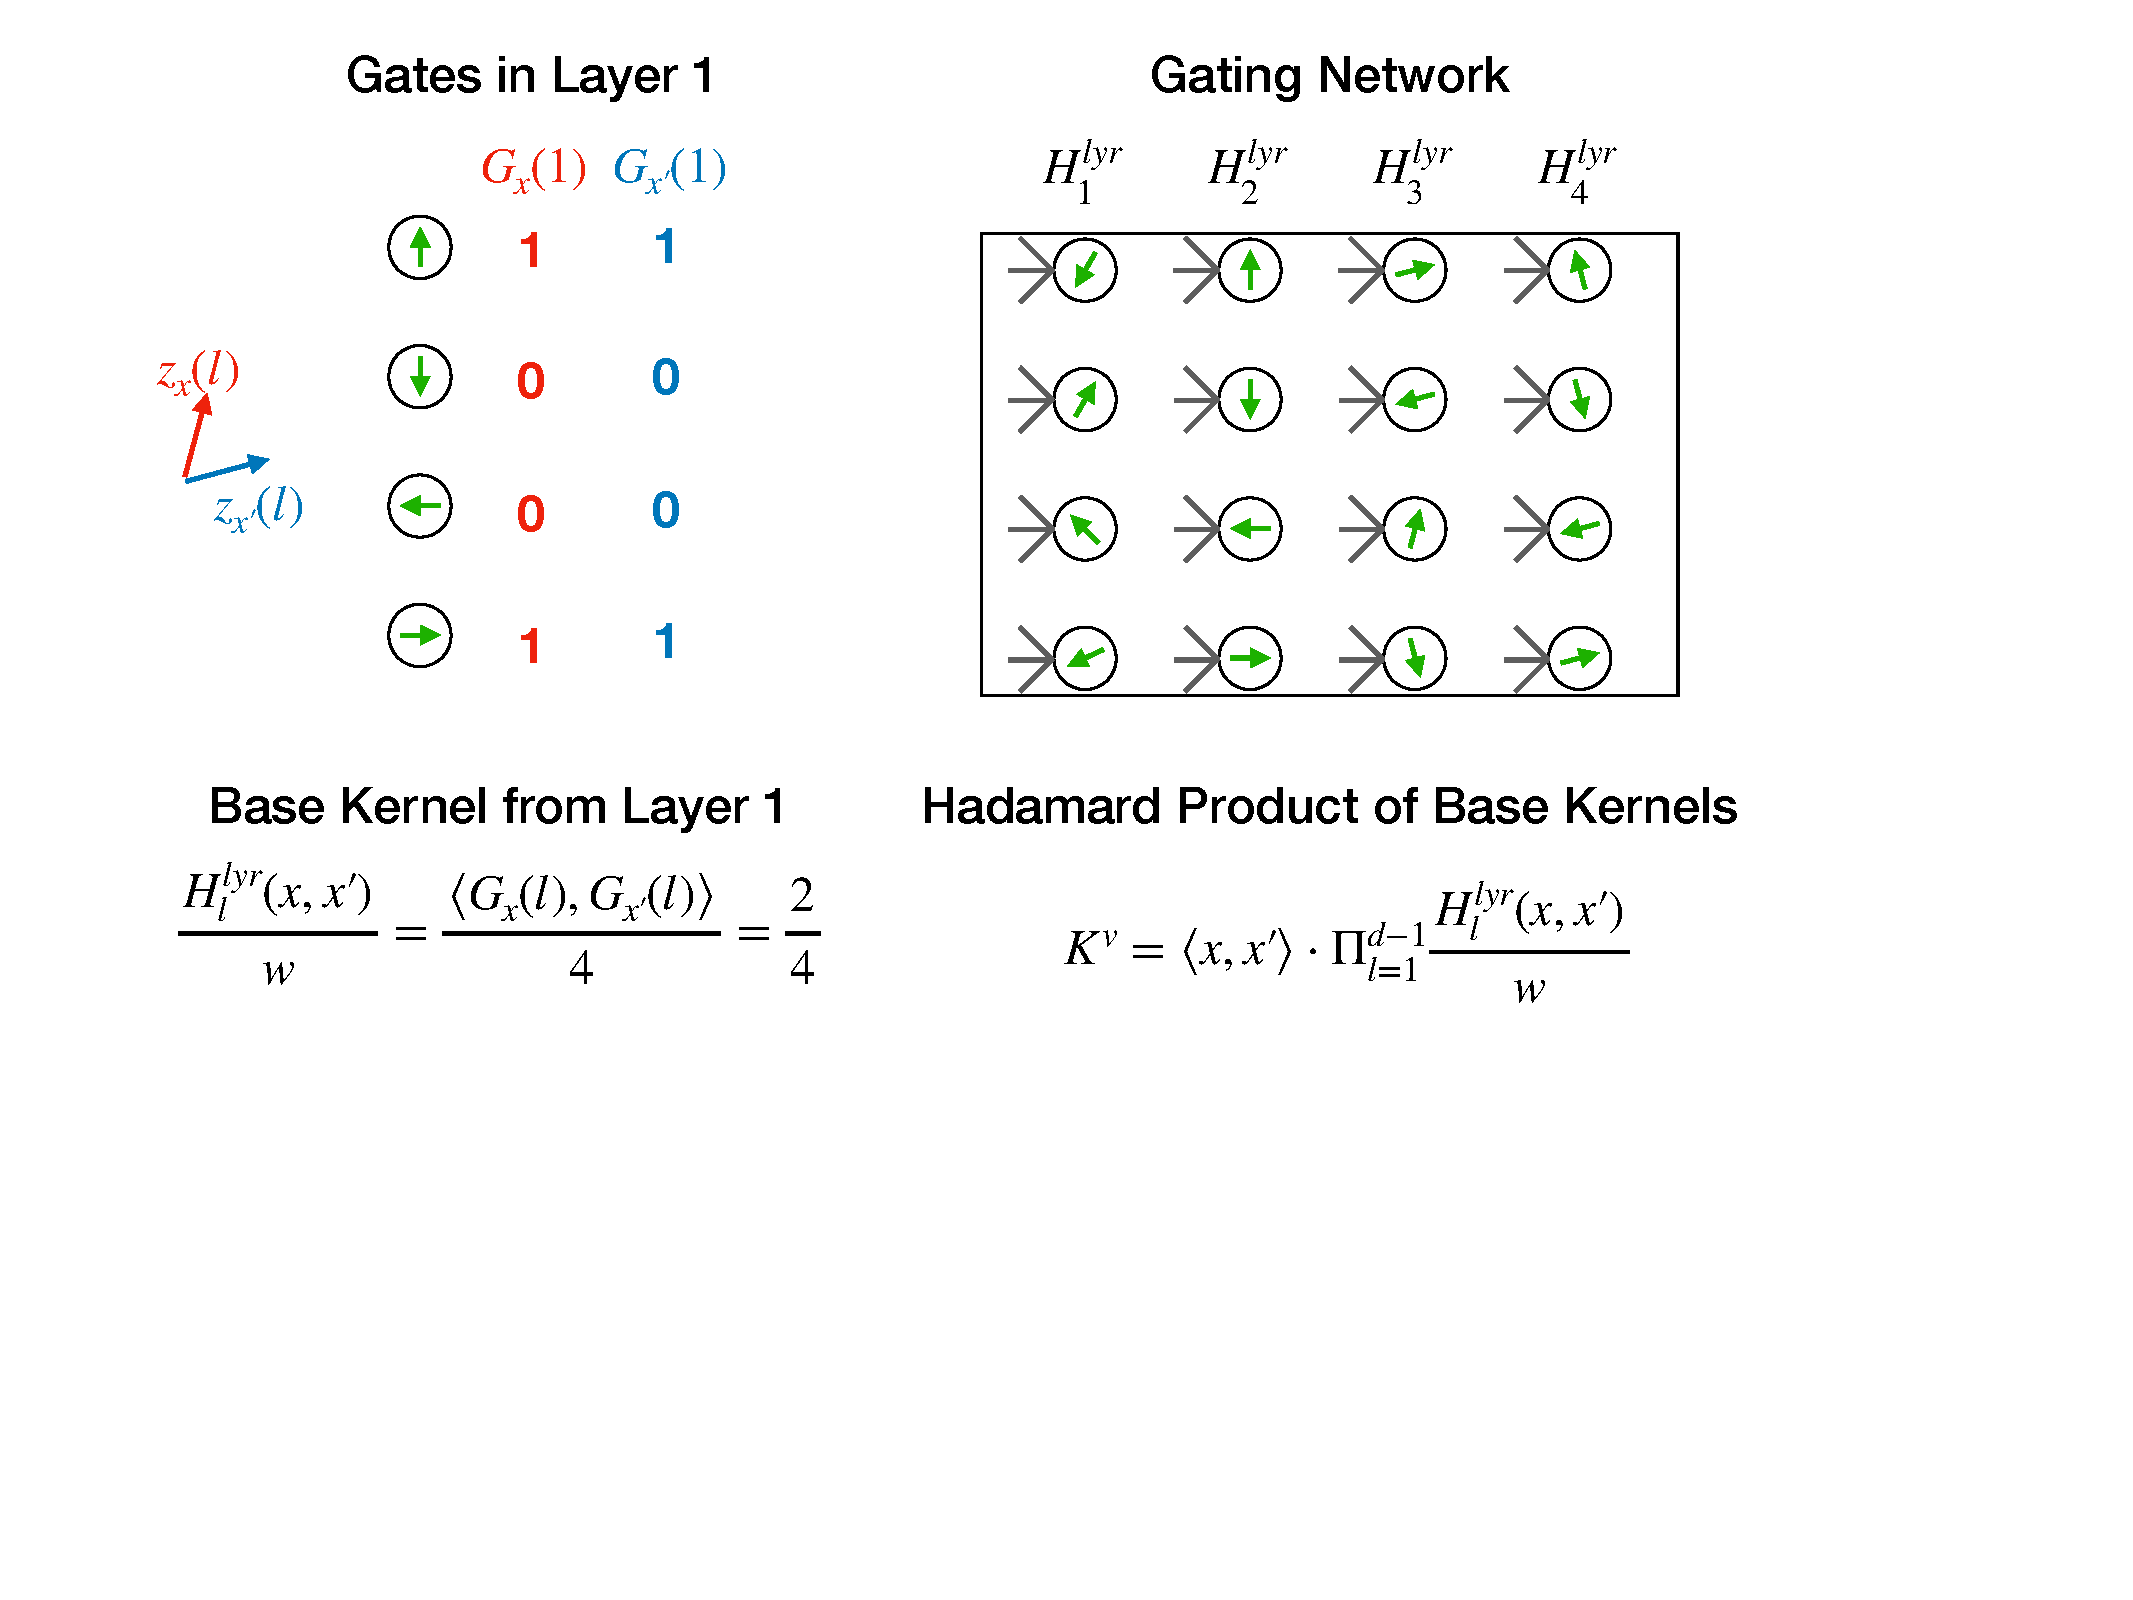
\includegraphics[scale=0.25]{figs/overall.pdf}
\end{figure}
\end{comment}
